%% uncomment to list all files in log
%\listfiles

\documentclass[12pt]{report}


\usepackage{fontspec}

%\setmainfont[Scale=MatchLowercase]{Lucida Bright}
%\setmonofont{FreeMono}
%\setmonofont{Source Code Pro}
\setmonofont[Scale=MatchLowercase]{Ubuntu Mono}

\usepackage[headings]{fullpage}

% national use characters 
%\usepackage{inputenc}

% ams mathematical symbols
\usepackage{amsmath,amssymb}

% added to support pandoc highlighting
\usepackage{microtype}

\usepackage{makeidx}

% add index and bibliographies to table of contents
\usepackage[nottoc]{tocbibind}

% postscript courier and times in place of cm fonts
%\usepackage{courier}
%\usepackage{times}

% extended coloring
\usepackage{color}
\usepackage[table,dvipsnames]{xcolor}
\usepackage{colortbl}

% advanced date formating
\usepackage{datetime}

%support pandoc code highlighting
\usepackage{fancyvrb}
\DefineShortVerb[commandchars=\\\{\}]{\|}
\DefineVerbatimEnvironment{Highlighting}{Verbatim}{commandchars=\\\{\}}
% Add ',fontsize=\small' for more characters per line

%tango style colors
% \usepackage{framed}
% \definecolor{shadecolor}{RGB}{255,255,255}
% \newenvironment{Shaded}{\begin{snugshade}}{\end{snugshade}}
% \newcommand{\KeywordTok}[1]{\textcolor[rgb]{0.13,0.29,0.53}{\textbf{{#1}}}}
% \newcommand{\DataTypeTok}[1]{\textcolor[rgb]{0.13,0.29,0.53}{{#1}}}
% \newcommand{\DecValTok}[1]{\textcolor[rgb]{0.00,0.00,0.81}{{#1}}}
% \newcommand{\BaseNTok}[1]{\textcolor[rgb]{0.00,0.00,0.81}{{#1}}}
% \newcommand{\FloatTok}[1]{\textcolor[rgb]{0.00,0.00,0.81}{{#1}}}
% \newcommand{\CharTok}[1]{\textcolor[rgb]{0.31,0.60,0.02}{{#1}}}
% \newcommand{\StringTok}[1]{\textcolor[rgb]{0.31,0.60,0.02}{{#1}}}
% \newcommand{\CommentTok}[1]{\textcolor[rgb]{0.56,0.35,0.01}{\textit{{#1}}}}
% \newcommand{\OtherTok}[1]{\textcolor[rgb]{0.56,0.35,0.01}{{#1}}}
% \newcommand{\AlertTok}[1]{\textcolor[rgb]{0.94,0.16,0.16}{{#1}}}
% \newcommand{\FunctionTok}[1]{\textcolor[rgb]{0.00,0.00,0.00}{{#1}}}
% \newcommand{\RegionMarkerTok}[1]{{#1}}
% \newcommand{\ErrorTok}[1]{\textbf{{#1}}}
% \newcommand{\NormalTok}[1]{{#1}}

%espresso style colors
% \usepackage{framed}
% \definecolor{shadecolor}{RGB}{42,33,28}
% \newenvironment{Shaded}{\begin{snugshade}}{\end{snugshade}}
% \newcommand{\KeywordTok}[1]{\textcolor[rgb]{0.26,0.66,0.93}{\textbf{{#1}}}}
% \newcommand{\DataTypeTok}[1]{\textcolor[rgb]{0.74,0.68,0.62}{\underline{{#1}}}}
% \newcommand{\DecValTok}[1]{\textcolor[rgb]{0.27,0.67,0.26}{{#1}}}
% \newcommand{\BaseNTok}[1]{\textcolor[rgb]{0.27,0.67,0.26}{{#1}}}
% \newcommand{\FloatTok}[1]{\textcolor[rgb]{0.27,0.67,0.26}{{#1}}}
% \newcommand{\CharTok}[1]{\textcolor[rgb]{0.02,0.61,0.04}{{#1}}}
% \newcommand{\StringTok}[1]{\textcolor[rgb]{0.02,0.61,0.04}{{#1}}}
% \newcommand{\CommentTok}[1]{\textcolor[rgb]{0.00,0.40,1.00}{\textit{{#1}}}}
% \newcommand{\OtherTok}[1]{\textcolor[rgb]{0.74,0.68,0.62}{{#1}}}
% \newcommand{\AlertTok}[1]{\textcolor[rgb]{1.00,1.00,0.00}{{#1}}}
% \newcommand{\FunctionTok}[1]{\textcolor[rgb]{1.00,0.58,0.35}{\textbf{{#1}}}}
% \newcommand{\RegionMarkerTok}[1]{\textcolor[rgb]{0.74,0.68,0.62}{{#1}}}
% \newcommand{\ErrorTok}[1]{\textcolor[rgb]{0.74,0.68,0.62}{\textbf{{#1}}}}
% \newcommand{\NormalTok}[1]{\textcolor[rgb]{0.74,0.68,0.62}{{#1}}}

%kete style colors
% \newenvironment{Shaded}{}{}
% \newcommand{\KeywordTok}[1]{\textbf{{#1}}}
% \newcommand{\DataTypeTok}[1]{\textcolor[rgb]{0.50,0.00,0.00}{{#1}}}
% \newcommand{\DecValTok}[1]{\textcolor[rgb]{0.00,0.00,1.00}{{#1}}}
% \newcommand{\BaseNTok}[1]{\textcolor[rgb]{0.00,0.00,1.00}{{#1}}}
% \newcommand{\FloatTok}[1]{\textcolor[rgb]{0.50,0.00,0.50}{{#1}}}
% \newcommand{\CharTok}[1]{\textcolor[rgb]{1.00,0.00,1.00}{{#1}}}
% \newcommand{\StringTok}[1]{\textcolor[rgb]{0.87,0.00,0.00}{{#1}}}
% \newcommand{\CommentTok}[1]{\textcolor[rgb]{0.50,0.50,0.50}{\textit{{#1}}}}
% \newcommand{\OtherTok}[1]{{#1}}
% \newcommand{\AlertTok}[1]{\textcolor[rgb]{0.00,1.00,0.00}{\textbf{{#1}}}}
% \newcommand{\FunctionTok}[1]{\textcolor[rgb]{0.00,0.00,0.50}{{#1}}}
% \newcommand{\RegionMarkerTok}[1]{{#1}}
% \newcommand{\ErrorTok}[1]{\textcolor[rgb]{1.00,0.00,0.00}{\textbf{{#1}}}}
% \newcommand{\NormalTok}[1]{{#1}}
%end pandoc code hacks

% jodliterate colors
\usepackage{color}
\definecolor{shadecolor}{RGB}{248,248,248}
% j control structures 
\definecolor{keywcolor}{rgb}{0.13,0.29,0.53}
% j explicit arguments x y m n u v
\definecolor{datacolor}{rgb}{0.13,0.29,0.53}
% j numbers - all types see j.xml
\definecolor{decvcolor}{rgb}{0.00,0.00,0.81}
\definecolor{basencolor}{rgb}{0.00,0.00,0.81}
\definecolor{floatcolor}{rgb}{0.00,0.00,0.81}
% j local assignments
\definecolor{charcolor}{rgb}{0.31,0.60,0.02}
\definecolor{stringcolor}{rgb}{0.31,0.60,0.02}
\definecolor{commentcolor}{rgb}{0.56,0.35,0.01}
% primitive adverbs and conjunctions
%\definecolor{othercolor}{rgb}{0.56,0.35,0.01}   
\definecolor{othercolor}{RGB}{0,0,255}
% global assignments
\definecolor{alertcolor}{rgb}{0.94,0.16,0.16}
% primitive J verbs and noun names
\definecolor{funccolor}{rgb}{0.00,0.00,0.00}    

\usepackage{framed}
\newenvironment{Shaded}{}{}
\newcommand{\KeywordTok}[1]{\textcolor{keywcolor}{\textbf{{#1}}}}
\newcommand{\DataTypeTok}[1]{\textcolor{datacolor}{{#1}}}
%\newcommand{\DecValTok}[1]{\textcolor{decvcolor}{{#1}}}
\newcommand{\DecValTok}[1]{{#1}} 
\newcommand{\BaseNTok}[1]{\textcolor{basencolor}{{#1}}}
\newcommand{\FloatTok}[1]{\textcolor{floatcolor}{{#1}}}
\newcommand{\CharTok}[1]{\textcolor{charcolor}{\textbf{{#1}}}}
\newcommand{\StringTok}[1]{\textcolor{stringcolor}{{#1}}}
\newcommand{\CommentTok}[1]{\textcolor{commentcolor}{\textit{{#1}}}}
\newcommand{\OtherTok}[1]{\textcolor{othercolor}{{#1}}} 
\newcommand{\AlertTok}[1]{\textcolor{alertcolor}{\textbf{{#1}}}}
%\newcommand{\FunctionTok}[1]{\textcolor{funccolor}{{#1}}}
\newcommand{\FunctionTok}[1]{{#1}}
\newcommand{\RegionMarkerTok}[1]{{#1}}
\newcommand{\ErrorTok}[1]{\textbf{{#1}}}
\newcommand{\NormalTok}[1]{{#1}}

% headers and footers
\usepackage{fancyhdr}
\pagestyle{fancy}

\fancyhead{}
\fancyfoot{}

%\fancyhead[LE,RO]{\slshape \rightmark}
%\fancyhead[LO,RE]{\slshape \leftmark}
\fancyfoot[C]{\thepage}
%\headrulewidth 0.4pt
%\footrulewidth 0 pt

%\addtolength{\headheight}{\baselineskip}

%\lfoot{\emph{Analyze the Data not the Drivel}}
%\rfoot{\emph{\today}}

% subfigure handles figures that contain subfigures
%\usepackage{color,graphicx,subfigure,sidecap}
\usepackage{graphicx,sidecap}
\usepackage{subfigure}
\graphicspath{{./inclusions/}}

% floatflt provides for text wrapping around small figures and tables
\usepackage{floatflt}

% tweak caption formats 
\usepackage{caption} 
\usepackage{sidecap}
%\usepackage{subcaption} % not compatible with subfigure

\usepackage{rotating} % flip tables sideways

% complex footnotes
%\usepackage{bigfoot}

% weird logos \XeLaTeX
\usepackage{metalogo}

% source code listings
\usepackage{listings}

% long tables
% \usepackage{longtable}

\newcommand{\HRule}{\rule{\linewidth}{0.5mm}}

% map LaTeX cross references into PDF cross references
\usepackage[
            %dvips,
            colorlinks,
            linkcolor=blue,
            citecolor=blue,
            urlcolor=blue,   % magenta, cyan default        
            pdfauthor={John D. Baker},
            pdftitle={Analyze the Data not the Drivel},
            pdfsubject={Blog},
            pdfcreator={MikTeX+LaTeXe with hyperref package},
            pdfkeywords={blog,wordpress},
            ]{hyperref}
           
% custom colors
\definecolor{CodeBackGround}{cmyk}{0.0,0.0,0,0.05}    % light gray
\definecolor{CodeComment}{rgb}{0,0.50,0.00}           % dark green {0,0.45,0.08}
\definecolor{TableStripes}{gray}{0.9}                 % odd/even background in tables

\lstdefinelanguage{bat}
{morekeywords={echo,title,pushd,popd,setlocal,endlocal,off,if,not,exist,set,goto,pause},
sensitive=True,
morecomment=[l]{rem}
}

\lstdefinelanguage{jdoc}
{
morekeywords={},
otherkeywords={assert.,break.,continue.,for.,do.,if.,else.,elseif.,return.,select.,end.
,while.,whilst.,throw.,catch.,catchd.,catcht.,try.,case.,fcase.},
sensitive=True,
morecomment=[l]{NB.},
morestring=[b]',
morestring=[d]',
}

% latex size ordering - can never remember it
% \tiny
% \scriptsize
% \footnotesize
% \small
% \normalsize
% \large
% \Large
% \LARGE
% \huge
% \Huge
 
% listings package settings  
\lstset{%
  language=jdoc,                                % j document settings
  basicstyle=\ttfamily\footnotesize,            
  keywordstyle=\bfseries\color{keywcolor}\footnotesize,
  identifierstyle=\color{black},
  commentstyle=\slshape\color{CodeComment},     % colored slanted comments
  stringstyle=\color{red}\ttfamily,
  showstringspaces=false,                       
  %backgroundcolor=\color{CodeBackGround},       
  frame=single,                                
  framesep=1pt,                                 
  framerule=0.8pt,                             
  rulecolor=\color{CodeBackGround},   
  showspaces=false,
  %columns=fullflexible,
  %numbers=left,
  %numberstyle=\footnotesize,
  %numbersep=9pt,
  tabsize=2,
  showtabs=false,
  captionpos=b
  breaklines=true,                              
  breakindent=5pt                              
}

\lstdefinelanguage{JavaScript}{
  keywords={typeof, new, true, false, catch, function, return, null, catch, switch, var, if, in, while, do, else, case, break},
  ndkeywords={class, export, boolean, throw, implements, import, this},
  ndkeywordstyle=\color{darkgray}\bfseries,
  sensitive=false,
  comment=[l]{//},
  morecomment=[s]{/*}{*/},
  morestring=[b]',
  morestring=[b]"
}

% C# settings
\lstdefinestyle{sharpc}{
language=[Sharp]C,
basicstyle=\ttfamily\scriptsize, 
keywordstyle=\bfseries\color{keywcolor}\scriptsize,
framerule=0pt
}

% for source code listing longer than two use smaller font
\lstdefinestyle{smallersource}{
basicstyle=\ttfamily\scriptsize, 
keywordstyle=\bfseries\color{keywcolor}\scriptsize,
framerule=0pt
}

\lstdefinestyle{resetdefaults}{
language=jdoc,
basicstyle=\ttfamily\footnotesize,  
keywordstyle=\bfseries\color{keywcolor}\footnotesize,                                                               
framerule=0.8pt 
}

% APL UTF8 code points listed for lstlisting processing
\makeatletter
\lst@InputCatcodes
\def\lst@DefEC{%
 \lst@CCECUse \lst@ProcessLetter
  ^^80^^81^^82^^83^^84^^85^^86^^87^^88^^89^^8a^^8b^^8c^^8d^^8e^^8f%
  ^^90^^91^^92^^93^^94^^95^^96^^97^^98^^99^^9a^^9b^^9c^^9d^^9e^^9f%
  ^^a0^^a1^^a2^^a3^^a4^^a5^^a6^^a7^^a8^^a9^^aa^^ab^^ac^^ad^^ae^^af%
  ^^b0^^b1^^b2^^b3^^b4^^b5^^b6^^b7^^b8^^b9^^ba^^bb^^bc^^bd^^be^^bf%
  ^^c0^^c1^^c2^^c3^^c4^^c5^^c6^^c7^^c8^^c9^^ca^^cb^^cc^^cd^^ce^^cf%
  ^^d0^^d1^^d2^^d3^^d4^^d5^^d6^^d7^^d8^^d9^^da^^db^^dc^^dd^^de^^df%
  ^^e0^^e1^^e2^^e3^^e4^^e5^^e6^^e7^^e8^^e9^^ea^^eb^^ec^^ed^^ee^^ef%
  ^^f0^^f1^^f2^^f3^^f4^^f5^^f6^^f7^^f8^^f9^^fa^^fb^^fc^^fd^^fe^^ff%
  ^^^^20ac^^^^0153^^^^0152%
  ^^^^20a7^^^^2190^^^^2191^^^^2192^^^^2193^^^^2206^^^^2207^^^^220a%
  ^^^^2218^^^^2228^^^^2229^^^^222a^^^^2235^^^^223c^^^^2260^^^^2261%
  ^^^^2262^^^^2264^^^^2265^^^^2282^^^^2283^^^^2296^^^^22a2^^^^22a3%
  ^^^^22a4^^^^22a5^^^^22c4^^^^2308^^^^230a^^^^2336^^^^2337^^^^2339%
  ^^^^233b^^^^233d^^^^233f^^^^2340^^^^2342^^^^2347^^^^2348^^^^2349%
  ^^^^234b^^^^234e^^^^2350^^^^2352^^^^2355^^^^2357^^^^2359^^^^235d%
  ^^^^235e^^^^235f^^^^2361^^^^2362^^^^2363^^^^2364^^^^2365^^^^2368%
  ^^^^236a^^^^236b^^^^236c^^^^2371^^^^2372^^^^2373^^^^2374^^^^2375%
  ^^^^2377^^^^2378^^^^237a^^^^2395^^^^25af^^^^25ca^^^^25cb%  
  ^^00}
\lst@RestoreCatcodes
\makeatother

% custom lengths used within minipages
\newcommand{\minindent}{17pt}


\makeindex

\begin{document}

\subsection*{\href{http://analyzethedatanotthedrivel.org/2020/08/03/neowise-nostalgia/}{Neowise Nostalgia}}
\addcontentsline{toc}{subsection}{Neowise Nostalgia}


\noindent\emph{Posted: 03 Aug 2020 21:47:46}
\vspace{6pt}

\href{https://en.wikipedia.org/wiki/C/2020_F3_(NEOWISE)}{Comet Neowise}
is fading fast. For the last two weeks, I've been watching Neowise climb
higher and higher in the early evening northwestern sky. Neowise was a
welcome sight in this shit-storm (2020) year. Gazing at its diffuse tail
takes your mind off the Wuhan
Coronavirus\footnote{I don't give a ding-dong-damn about whether you think Winnie the
  Chinese Wuhan Coronavirus is racist or not. The virus \emph{cannot}
  care about what it's called, and neither should you. Ignore the
  \href{https://www.baltimoresun.com/opinion/op-ed/bs-ed-op-0630-wokerati-20190620-story.html}{\emph{wokerati}};
  for them everything is racist. They've stripped the word ``racist'' of
  its meaning.
  \href{https://www.goodreads.com/quotes/553001-it-s-a-beautiful-thing-the-destruction-of-words-of-course}{``It's a beautiful thing, the destruction of words.''}} and the global,
mostly self-inflicted, economic clusterfuck it caused.

In 16x70 binoculars Neowise was a fine sight; its bifurcated tail
spanned the entire field of view but, without binoculars, Neowise was a
dud for my cataract compromised eyes. Despite my best
\emph{averted-vision} efforts I never saw it without binoculars. So, as
fine as Neowise was, it comes in last on my lifetime comet list. For a
longtime amateur astronomer, my lifetime comet list is embarrassingly
short. Here it is:

\medskip

\noindent \textbf{Comet Bennet 1970 near Canmore Alberta Canada}

\medskip

My first naked eye comet was a complete surprise. I was returning from a
spring break Vancouver trip with two, now deceased, friends, Carl
Sullivan and Lawrence Nazar. It was past midnight, we had just driven
through Banff National Park on the way to Calgary when we pulled over to
pee. While pissing on crusty highway shoulder snow we looked up at the
mountains to the south. Shining high above the dark peaks was the most
beautiful comet I've ever seen. At the time we didn't know the comet's
name and we weren't entirely sure it was a comet. It was just too
perfect! It looked exactly like a textbook comet. Later, another friend
Bob Blaxley identified the apparition:
\href{https://en.wikipedia.org/wiki/Comet_Bennett}{comet Bennet}. We saw
Bennet under nearly ideal conditions. The sky was pitch black and the
comet was very high. The tail was spectacular.

\medskip

\noindent \textbf{Haley's Comet 1986 Edmonton Alberta Canada}

\medskip

\href{https://en.wikipedia.org/wiki/Halley's_Comet}{Haley's Comet} is
easily the most famous comet out there. It's the one comet every
literate person knows. Haley is a short-period comet. It famously
returns every 75 to 76 years. Haley's human lifetime period
distinguishes it from most comets. If you're lucky you can see Haley's
Comet twice. Mark Twain often opined that he came in with Haley's Comet
and expected to go out with it.
\href{http://www.todayifoundout.com/index.php/2013/10/samuel-clemens-born-died-year-halleys-comet/}{He
did!} Contrast this with Neowise. It won't return for another 6,700
years. Nobody alive today will witness Neowise's return. Hell, even
Bristlecone Pines, trees that can live up to 5,000 years, won't see
Neowise again.

Some of Haley's passes have been spectacular. The 1910 pass was
impressive, but the 1986 pass was a dud. In 1986 Haley's Comet was far
from Earth and appeared as a small fuzzy tailless spot in Edmonton
Alberta's skies. I'm glad I caught Haley's in 1986. I doubt I'll see it
again in 2061.

\medskip

\noindent \textbf{Comet Hyakutake 1996 Kingston Ontario Canada}

\medskip

In 1996 we were all holding our breath as Hale Bopp approached
perihelion. Hale Bopp had been discovered way out and we were hoping it
would blossom into the bright enduring comet we craved. We had been
bitterly disappointed before; we shall not utter
\href{https://en.wikipedia.org/wiki/Comet_Kohoutek}{Kohoutek}'s name.
With Hale Bopp on the way,
\href{https://en.wikipedia.org/wiki/Comet_Hyakutake}{Hyakutake} was seen
as a warm-up act. But, just like warm-up bands can out-play headliners,
Hyakutake, the little comet that could, put on a great show.

On the week of Hyakutake's closet approach to Earth, I was eagerly
looking for it but Kingston Ontario's crappy cloudy skies got in the
way. Every night, for a week, I gazed up at the butt-holes of clouds not
exactly the tail\footnote{How's that for \emph{micro-aggressive} comet sexual
 innuendo? } I was
looking for. The weather was grim, unrelenting, savage, cruel,
relentless; it almost broke me, but then one night, as I was pulling
into our driveway I looked up and saw perfectly framed in a cloud gap
the long twisty filamentary tail of Hyakutake. The tail spread over
twenty degrees. It was the longest comet tail I have ever seen. The
following evening Kingston's skies clouded out and I never saw Hyakutake
again.

\medskip

\noindent \textbf{Hale Bopp 1997 Kingston Ontario Canada}

\medskip

You could make a good case that
\href{https://en.wikipedia.org/wiki/Comet_Hale\%E2\%80\%93Bopp}{Hale
Bopp} was the comet of the 20\textsuperscript{th} century. Most naked
eye comets show for a few weeks; Hale Bopp graced Earth's skies for over
a year. Hale Bopp was easily visible to anyone that bothered looking up
in 1997. It hung around for so long that we almost got
bored\footnote{It takes a special type of asshole to be bored by a comet.
} with it! As grand as
Hale Bopp was it could have been beyond epic. Like Haley's Comet in 1986
Hale Bopp was very far from the Earth when it zoomed by, but unlike
Haley's which appeared as a small fuzzy blob, Hale Bopp glowed like the
much closer Bennet for months. If Hale Bopp had passed as close to Earth
as Hyakutake had people would have lost their apocalyptic shit!

%\begin{figure}
%\centering
%\includegraphics[width=2.61458in,height=1.73958in]{https://bakerjd99.files.wordpress.com/2020/08/heavens_gate_suicides.jpg}
%\caption{Not the best posture for comet viewing but you have to respect
%the Nike product placement.}
%\end{figure}

% captions beside figure
\captionsetup[figure]{labelformat=empty}
\begin{SCfigure}
\centering
\includegraphics[width=0.30\textwidth]{heavens_gate_suicides.jpg}
\caption[Not the best posture for comet viewing]{Not the best posture for comet viewing but you have to respect
the Nike product placement.}
\label{fig:6024x0}
\end{SCfigure}

Some, too stupid to live, morons lost their apocalyptic shit anyway!
Remember the
\href{https://www.escondidograpevine.com/2020/03/25/20-years-ago-heavens-gate-couldnt-wait/}{Heaven's
Gate} suicide squad that boarded spaceship Hale Bopp with phenobarbital?
I'll never forget their little
\href{https://solecollector.com/news/2015/03/nike-decade-heavens-gate-sneakers}{Nike}
clad feet sticking out from under their purple death sheets. Ahh, good
times!

\medskip

\noindent \textbf{Comet Neowise Meridian Idaho United States}

\medskip

Neowise is the last comet on my list. It didn't put on a grand show or
inspire any suicidal death cults but I'll miss it anyway. Bon Voyage
Neowise.

%\begin{center}\rule{0.5\linewidth}{0.5pt}\end{center}
%
%\begin{center}\rule{0.5\linewidth}{0.5pt}\end{center}
%
%\begin{enumerate}
%\item
%  \leavevmode\hypertarget{fn1}{}%
%  I don't give a ding-dong-damn about whether you think Winnie the
%  Chinese Wuhan Coronavirus is racist or not. The virus \emph{cannot}
%  care about what it's called, and neither should you. Ignore the
%  \href{https://www.baltimoresun.com/opinion/op-ed/bs-ed-op-0630-wokerati-20190620-story.html}{\emph{wokerati}};
%  for them everything is racist. They've stripped the word ``racist'' of
%  its meaning.
%  \href{https://www.goodreads.com/quotes/553001-it-s-a-beautiful-thing-the-destruction-of-words-of-course}{``It's
%  a beautiful thing, the destruction of
%  words.''}\protect\hyperlink{fnref1}{↩︎}
%\item
%  \leavevmode\hypertarget{fn2}{}%
%  How's that for \emph{micro-aggressive} comet sexual
%  innuendo?\protect\hyperlink{fnref2}{↩︎}
%\item
%  \leavevmode\hypertarget{fn3}{}%
%  It takes a special type of asshole to be bored by a
%  comet.\protect\hyperlink{fnref3}{↩︎}
%\end{enumerate}



%\end{document}
 
% standard floating figure
% \captionsetup[figure]{labelformat=empty}
% \begin{figure}[htbp]
% \centering
% \href{}{\includegraphics[width=0.50\textwidth]{}}
% \caption{}
% \label{fig:????x0}
% \end{figure}
 
% captions beside figure
% \captionsetup[figure]{labelformat=empty}
% \begin{SCfigure}
% \centering
% \href{}{\includegraphics[width=0.40\textwidth]{}}
% \caption{}
% \label{fig:????x0}
% \end{SCfigure}
 
